\section{Caminos y Ciclos}

Este tema ya lo motivamos con el ejemplo de los puentes de K\"onigsberg de la sección anterior.
En esta sección nos interesará estudiar algunas propiedades importantes de los grafos que tienen que ver con \emph{caminos} y \emph{ciclos} sobre ellos.
Comenzaremos con un par de definiciones importantes para nuestro siguiente estudio.

\begin{definicion}
Una {\bf caminata} en un grafo (no necesariamente simple) $G$ es una secuencia de vértices y aristas  $(v_0,e_1,v_1,e_2,v_2,\ldots,e_k,v_k)$ tal que para $1\leq i\leq k$, la arista $e_i$ une a los vértices $v_{i-1}$ y $v_i$.
Una {\bf caminata cerrada} en un grafo es una caminata en la que el primer y último vértices son iguales ($v_0=v_k$).
Cuando el grafo es simple, se pueden omitir los nombres de las aristas entre vértices en la representación de una caminata.

Un {\bf camino} en un grafo $G$, es una caminata en la que no se repiten aristas.
Un {\bf ciclo} en un grafo $G$, es una caminata cerrada en la que no se repiten aristas.
(Estas definiciones no debieran causar confusión con las definiciones de $P_n$ y $C_n$ que son clases de grafos, aquí estamos definiendo camino y ciclo \emph{en un grafo dado}, son subgrafos de un grafo dado.)

Una caminata o camino que comience en $u$ y termine en $v$ lo llamaremos caminata $u-v$ o camino $u-v$.
El largo de una caminata, caminata cerrada, camino y ciclo, se obtiene a partir de la cantidad de aristas.
Por simplicidad supondremos que un camino (o ciclo, o caminata) de largo $0$ es un camino (o ciclo o caminata) compuesto por un único vértice sin aristas.
\end{definicion}

\begin{ejemplo}
En el grafo de la figura~\ref{fig:graph16-b} las secuencia:
\begin{figure}[h!]
\centering
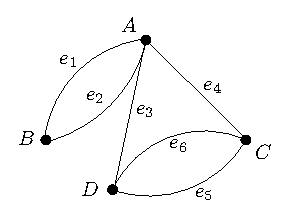
\includegraphics{graph16}
\caption{Grafo sin rulos}
\label{fig:graph16-b}
\end{figure}
\begin{itemize} 
  \itemsep 0pt
  \item $(D,e_6,C,e_5,D,e_6,C,e_4,A,e_1,B,e_1,A)$ es una caminata pero no un camino, su largo es 6.
  \item $(D,e_6,C,e_5,D,e_6,C,e_4,A,e_1,B,e_1,A)$ es una caminata cerrada pero no un ciclo., su largo es 6.
  \item $(D,e_6,C,e_5,D,e_3,A,e_2,B)$ es un camino, su largo es $4$.
  \item $(D,e_6,C,e_5,D,e_3,A,e_2,B,e_1,A,e_3,D)$ es un ciclo, su largo es $6$.
  \item $(D,e_3,B,e_1,C)$ no es una caminata.
\end{itemize}
En ellos es necesario nombrar las aristas dado que el grafo no es simple.

En el grafo simple de la figura~\ref{fig:graph17} podemos decir que las secuencias:
\begin{figure}[h!]
\centering
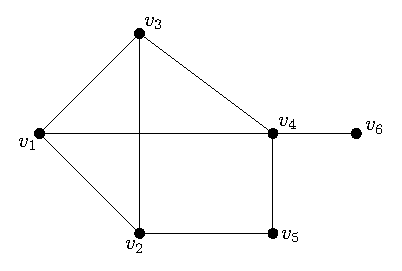
\includegraphics{graph17}
\caption{Grafo simple}
\label{fig:graph17}
\end{figure}
\begin{itemize}
  \itemsep 0pt
  \item $(v_1,v_4,v_5,v_2,v_3,v_4,v_5)$ es una caminata pero no un camino, su largo es $6$.
  \item $(v_1,v_4,v_5,v_2,v_3,v_4,v_5,v_4,v_1)$ es una caminata cerrada pero no un camino, su largo es $8$.
  \item $(v_1,v_4,v_6)$ es un camino, su largo es $3$.
  \item $(v_1,v_2,v_5,v_4,v_3,v_1)$ es un ciclo, su largo es $5$.
  \item $(v_1,v_5,v_6)$ no es una caminata.
\end{itemize}
En este caso no se nombran las arista ya que quedan implícitas por el hecho de sur un grafo simple.
\end{ejemplo}

\subsection{Conectividad}
\begin{definicion}
Un grafo $G$ se dice {\bf conexo} si para cada par de vértices $u,v\in V(G)$ existe un camino que contiene tanto a $u$ como a $v$.
No es difícil notar que si existe un camino que contiene a un par de vértices $u$ y $v$, entonces existe un camino cuyo vértice inicial es $u$ y final es $v$.
Cuando esto ocurra lo denotaremos por $u\sim v$.
La relación $\sim$, o como la llamaremos ``existe un camino entre'', es una relación de equivalencia sobre los vértices de un grafo.
A un grafo que no sea conexo le llamaremos disconexo.

Dado un grafo $G$, el subgrafo de $G$ compuesto por todos los caminos que contienen un vértice particular se llama {\bf componente conexa} de $G$.
La componente conexa de $G$ a la que pertenece un vértice $v$ particular, contiene a todos los vértices de $G$ que están relacionados con $v$ mediante $\sim$, es decir, todos los vértices de la clase de equivalencia de $v$.
\end{definicion}

\begin{ejemplo}
En la figura~\ref{fig:conex}, $G_1$ es un grafo conexo, mientras que $G_2$ no es conexo, por ejemplo no existe un camino entre los vértices $v_1$ y $v_8$.
En la misma figura, $G_2$ tiene $3$ componentes conexas, $\{v_2,v_6\}$, $\{v_1,v_3,v_5,v_7,v_9\}$, $\{v_4,v_8,v_{10}\}$.
En la figura~\ref{fig:conex-components} se ha dibujado $G_2$ de manera de mostrar claramente sus componentes conexas.
\begin{figure}[h!]
\centering
\begin{tabular}{cccc}
\includegraphics{graph18} & & & \includegraphics{graph19} \\
$G_1$ & & & $G_2$
\end{tabular}
\caption{$G_1$ es un grafo conexo, mientras que $G_2$ no lo es.}
\label{fig:conex}
\end{figure}
\begin{figure}[h!]
\centering
\includegraphics{graph20}
\caption{Componentes conexas de $G_2$.}
\label{fig:conex-components}
\end{figure}
\end{ejemplo}

>Cuántas aristas puedo agregarle al grafo $G_2$ de la figura~\ref{fig:conex-components} de tal manera que este siga siendo simple y teniendo tres componentes conexas?
>Cuántas aristas puedo sacar de $G$ de manera que este siga teniendo tres componentes conexas?
No es difícil notar que una nueva arisita agregada a un grafo puede disminuir la cantidad de componentes conexas a lo más en $1$, no las modifica si la arista es entre vértices de una misma componente y une dos componentes si la arista es entre vértices de distintas componentes.
De la misma forma, sacar una arista de un grafo puede aumentar la cantidad de componentes conexas a lo más en $1$.
Estas observaciones nos ayudan en el siguiente teorema.

\begin{teorema}\label{teo:min-components}
Un grafo $G$ con $n$ vértices y $k$ aristas tiene al menos $n-k$ componentes conexas.

\begin{demostracion}
Un grafo $G$ con $n$ vértices puede tener como máximo $n$ componentes conexas, cuando no tiene ninguna arista, cada nueva arista que se le agregue puede reducir la cantidad de componentes a lo más en $1$, por lo que luego de agregar $k$ aristas la cantidad de componentes se ha reducido como mínimo a $n-k$, por lo que la cantidad de componentes siempre se mantiene mayor o igual a $n-k$.
\end{demostracion}
\end{teorema}

El anterior teorema implica que si se quiere un grafo conexo de $n$ vértices, entonces al menos $n-1$ aristas son necesarias.
Una definición motivada también por la discusión anterior es la siguiente.

\begin{definicion}
Una {\bf arista de corte} en un grafo $G$ es una arista tal que su eliminación aumenta la cantidad de componentes.
Escribiremos $G-e$ para representar al grafo que resulta de eliminar la arista $e$ a $G$.

Un {\bf vértice de corte} en un grafo $G$ es un vértice tal que su eliminación aumenta la cantidad de componentes. 
Al eliminar un vértice $v$ de un grafo, sacamos $v$ y todas sus aristas incidentes, al grafo resultante lo llamamos $G-v$.
\end{definicion}

\begin{ejemplo}
En el grafo $G_1$ de la figura~\ref{fig:conex}, todas las aristas son de corte, y sus vértices de corte son $v_2,v_3,v_4,v_5,v_7,v_9$.
Un grafo como $G_1$ en el que todas sus aristas son de corte, es un grafo bien particular y lo estudiaremos en la siguiente sección.
En el grafo $G_2$ de la figura~\ref{fig:conex} no hay vértices de corte, y la única arista de corte es $v_2v_6$.
\end{ejemplo}

\begin{ejemplo}
Las aristas y vértices de corte así como la conectividad son conceptos muy importantes a la hora de diseñar una red (o grafo) de comunicación, como una red de computadores que intercambian datos, una red de repetidores de telefonía, o incluso una red de conexiones de vuelo entre ciudades (aquí lo comunicado serían pasajeros entre ciudades).

Tomemos el ejemplo de una red de computadores en la que necesitamos que todos los terminales sean capaces de comunicarse entre sí.
En el grafo asociado a esta red, cada vértice representa a un computador y una arista al cable que conecta un par de computadores.
La primera observación es que este grafo debe ser conexo para que todos los computadores puedan establecer comunicación.
>Que pasa si este grafo tiene algún vértice de corte?
Esto significaría que existe algún computador que, de fallar, haría imposible la comunicación entre algunos de los computadores que no han fallado.
>Qué pasa si este grafo tiene una arista de corte?
Esto significaría que existe alguna conexión (cable) que de fallar haría imposible la comunicación entre alguno de los computadores de la red.
Es interesante que al diseñar una red con un grafo asociado que no tenga ni puntos de corte ni aristas de corte, esta red será automáticamente \emph{tolerante a la falla} de un computador o un cable de comunicación.

En el ejemplo de los vuelos entre ciudades, en el grafo asociado cada vértice representaría a un aeropuerto en alguna ciudad, y una arista representaría la existencia de algún vuelo directo entre un par de aeropuertos.
Si existe un vértice de corte, querría decir que existe un aeropuerto que de ser cerrado dejará a algunas personas sin poder viajar por avión a su destino.
Algo similar pasa con las aristas de corte en este caso.
\end{ejemplo}

Caracterizaremos una arista de corte en términos de ciclos en el grafo.

\begin{teorema}\label{teo:cut-edge}
Una arista en un grafo $G$ es de corte si y sólo si no pertenece a ningún ciclo en $G$.

\begin{demostracion}
Nos centraremos en un grafo $G$ conexo, la demostración se aplicará entonces para cada componente conexa de $G$.

Sea $e=uv$ una arista que pertenece a un ciclo $C$ en $G$, al eliminar $e$ los únicos caminos afectados en $G-e$ son los que contenían a la arista $e=uv$, pero dado que esta pertenece a un ciclo $C$, los caminos afectados pueden completarse con la porción restante de $C$, luego la arista $e$ no puede ser de corte.

Supongamos ahora que $e=uv$ no es una arista de corte, o sea que $G-e$ sigue siendo conexo, esto quiere decir que existe un camino digamos $P$ entre $u$ y $v$ en $G-e$.
El camino $P$ junto con la arista $uv$ forman un ciclo en $G$.

\begin{figure}[h!]
\centering
\hspace*{6em}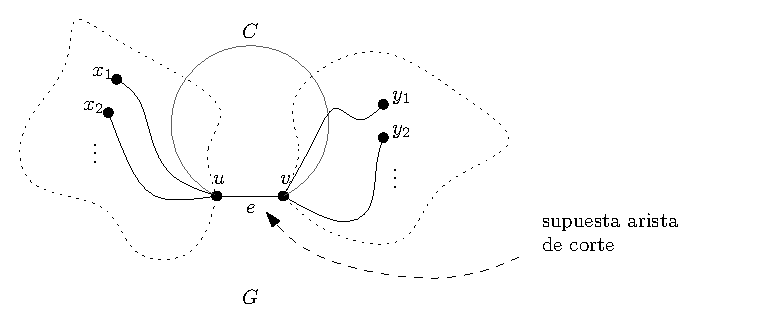
\includegraphics{cut-edge}
\caption{Una arista es de corte sólo si no pertenece a un ciclo.}
\label{fig:cut-edge}
\end{figure}
La idea central de la demostración se ve en la figura~\ref{fig:cut-edge}, claramente si $e=uv$ pertenece a un ciclo su eliminación no desconectará a $G$.
\end{demostracion}
\end{teorema}

\begin{ejemplo}
En el grafo $G_1$ de la figura~\ref{fig:conex}, ninguna de sus aristas pertenece a un ciclo ya que $G_1$ no tiene ningún ciclo, luego todas sus aristas son de corte.
En el grafo $G_2$ de la misma figura, la única arista que no pertenece a un ciclo es $v_2v_6$ por lo tanto es la única arista de corte.
\end{ejemplo}


\subsection{Grafos Bipartitos}
En esta sección estudiaremos una caracterización de grafos bipartitos en función de ciclos y caminos.

\begin{lema}\label{teo:odd-walk}
En un grafo simple $G$, toda caminata cerrada de largo impar, contiene un ciclo de largo impar.

\begin{demostracion}
Lo haremos usando un argumento inductivo en el largo de la caminata cerrada.
La caminata cerrada más pequeña de largo impar que se puede hacer en un grafo simple es un ciclo de tres vértices, esta caminata ya es un ciclo así que el caso base se comprueba.
Ahora tomemos una caminata $C$ cerrada de largo $l$ impar y supongamos como hipótesis de inducción que toda caminata cerrada de largo impar menor a $l$ tiene un ciclo de largo impar.
Si en $C$ no se repiten vértices entonces $C$ ya es un ciclo de largo impar y comprobamos lo que queríamos, si por otro lado en $C$ se repite un vértice, digamos $v$, entonces podemos partir $C$ en dos caminatas cerradas distintas que comienzan en $v$, $C'$ y $C''$ como se muestra en la figura~\ref{fig:odd-walk}.
\begin{figure}[h!]
\centering
\includegraphics{odd-walk}
\caption{Una caminata cerrada que repite un vértice, dividida en dos caminatas cerradas}
\label{fig:odd-walk}
\end{figure}
No puede ocurrir que simultáneamente $C'$ y $C''$ tengan largo par ya que entonces $C$ no podría tener largo impar, por lo que al menos una de ellas es una caminata cerrada de largo impar estrictamente menor a $l$ y por HI contiene un ciclo de largo impar, que también será un ciclo de largo impar contenido en $C$ comprobando lo que queríamos.
\end{demostracion}
\end{lema}

El anterior teorema sólo se aplica para caminatas cerradas de largo impar, una caminata cerrada de largo par podría no contener un ciclo de largo par, por ejemplo podría ser una caminata que repitiera todas las aristas dos veces cada una.
El anterior lema nos servirá para demostrar el siguiente teorema.

\begin{teorema}\label{teo:odd-cycle}
Un grafo conexo (simple) $G$  es bipartito si y sólo si no contiene ningún ciclo de largo impar.

\begin{demostracion}
$(\Rightarrow)$ Supongamos que $G$ contiene un ciclo de largo impar, digamos $C=(v_1,v_2,\ldots,v_{k-1},v_k,v_1)$, con $k$ un natural impar, demostraremos que $G$ no puede ser bipartito.
Supongamos que $G$ es bipartito con particiones $V_1$ y $V_2$ y supongamos sin pérdida de generalidad que $v_1\in V_1$.
Dado que $C$ es un ciclo, necesariamente $v_iv_{i+1}\in E(G)$ para $1\leq i< k$ y $v_kv_1\in E(G)$, por lo que debe ocurrir que $v_2\in V_2$, $v_3\in V_1$, $v_4\in V_2$, etc. 
En general debe ocurrir que para los vértices del ciclo $C$, $v_i\in V_1$ si $i$ es impar, y $v_i\in V_2$ si $i$ es par, luego $v_k\in V_1$ lo que es una contradicción con el hecho de suponer que $V_1$ es una partición que contiene a $v_1$ ya que $v_kv_1\in E(G)$.

$(\Leftarrow)$ Supongamos que $G$ no contiene ningún ciclo de largo impar, demostraremos que es posible definir una partición de los vértices de $G$ en dos conjuntos independientes.
Sea $v$ un vértice cualquiera de $V(G)$, definimos $V_1=\{u\in V(G)\;|\;$ existe un camino de largo impar de $v$ a $u\}$, y $V_2=\{u\in V(G)\;|\;$ existe un camino de largo par de $v$ a $u\}$.
Si existiera una arista entre dos vértices de $V_1$ digamos $u_1$ y $u_2$, entonces, dado que existen caminos $v-u_1$ y $v-u_2$ ambos de largo impar, existiría una caminata cerrada de largo impar formada por los dos caminos anteriores más la arista $v_1v_2$ y por el lema~\ref{teo:odd-walk} existiría un ciclo de largo impar contradiciendo nuestra suposición.
Si existiera una arista entre dos vértices de $V_2$ digamos $w_1$ y $w_2$, entonces, dado que existen caminos $v-w_1$ y $v-w_2$ ambos de largo par, existiría una caminata cerrada de largo impar formada por los dos caminos anteriores más la arista $w_1w_2$ y nuevamente por el lema~\ref{teo:odd-walk} existiría un ciclo de largo impar contradiciendo nuestra suposición.
Finalmente no existe arista entre vértices de $V_1$ y no existe aristas entre vértices de $V_2$ y como $G$ es conexo se tiene que $V_1\cup V_2=V(G)$ por lo que $G$ es bipartito con particiones $V_1$ y $V_2$.
\end{demostracion}
\end{teorema}

No es difícil notar que si $G$ no es conexo pero si bipartito, la demostración se aplica a cada componente conexa, y también ocurrirá que $G$ no tendrá ciclos de largo impar.
Para demostrar entonces que un grafo $G$ es bipartito basta dividir los vértices de $G$ en dos conjuntos independientes.
Para demostrar que un grafo $G$ no es bipartito basta encontrar un ciclo de largo impar en $G$.

El alumno podría diseñar un algoritmo para determinar si un grafo es o no bipartito.
El algoritmo debiera ser tal que si el grafo es bipartito entonces el output entregue los conjuntos de vértices que conforman cada partición, y si el grafo no es bipartito el output entregue una secuencia de vértices que formen un ciclo de largo impar en el grafo.

\subsection{Ciclos y Caminos Eulerianos}
En el ejemplo de los puentes de K\"onigsberg los habitantes del pueblo querían encontrar una forma de recorrer la ciudad pasando una vez por cada puente y volviendo al lugar inicial.
Modelamos el problema usando un grafo y dijimos que el problema era equivalente a intentar ``dibujar'' el grafo sin repetir las aristas y volviendo al vértice de donde se inició el dibujo.
Ya argumentamos que si algún vértice del grafo tenía grado impar entonces tal dibujo no se podía lograr.
En esta sección completaremos el resultado, demostrando que esta condición es también suficiente para que un grafo pueda dibujarse siguiendo las restricciones, o sea que un grafo se puede dibujar sin repetir trazos y volviendo al vértice inicial, si y sólo si ninguno de sus vértices tiene grado impar.
Iniciaremos formalizando algunos conceptos.


\begin{definicion}
Un {\bf ciclo Euleriano} en un grafo $G$, es un ciclo que contiene a todas las aristas de $G$ y a todos los vértices de $G$.
Note que es importante que en un ciclo no se repitan aristas, pero perfectamente pueden repetirse vértices.
Diremos que $G$ es un {\bf grafo Euleriano} si contiene un ciclo Euleriano.
\end{definicion}

Según la definición anterior, el problema de los puentes de K\"onigsberg es equivalente a determinar si su grafo asociado es o no Euleriano.
En la figura~\ref{fig:graph21} se muestra un grafo que si es Euleriano, de hecho contiene el siguiente ciclo Euleriano: $(v_1,v_2,v_6,v_7,v_3,v_9,v_{10},v_4,v_8,v_9,v_5,v_7,v_1)$.

\begin{figure}[h!]
\centering
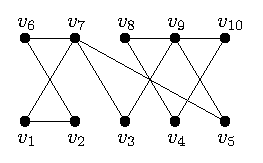
\includegraphics{graph21}
\caption{Grafo Euleriano.}
\label{fig:graph21}
\end{figure}

Estableceremos ahora el teorema importante de esta sección.

\begin{teorema}\label{teo:euler}
Un grafo $G$ (sin rulos) es Euleriano si y sólo si es conexo y todos sus vértices tienen grado par.

\begin{demostracion}
$(\Rightarrow)$ Supongamos que $G$ es Euleriano, entonces $G$ tiene un ciclo que contiene a todas las aristas y todos los vértices, supongamos que este ciclo parte (y termina) en un vértice particular $v$.
El ciclo necesita una arista para ``salir'' de $v$ y otra para ``llegar'' finalmente a $v$, y cada vez que $v$ aparece nuevamente en el ciclo necesita dos aristas distintas más (una para entrar y otra para salir), un diagrama se ve en la figura~\ref{fig:graph22}.
\begin{figure}[h!]
\centering
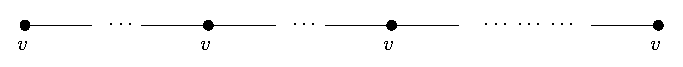
\includegraphics{graph22}
\caption{Un vértice $v$ particular del ciclo Euleriano y sus artistas incidentes.}
\label{fig:graph22}
\end{figure}
Esto implica que $\delta(v)$ necesariamente es par, ya que todas sus aristas incidentes aparecen en este ciclo una vez cada una.
Este ciclo se puede pensar que parte (y termina) en cada uno de los otros vértices del grafo concluyendo que todos tienen grado par.
Es claro también que si existe tal ciclo, el grafo $G$ es conexo ya que dentro del mismo ciclo se pueden encontrar caminos entre todos los pares de vértices de $G$.

$(\Leftarrow)$ Supongamos que $G$ es conexo y que todos sus vértices tiene grado par.
Demostraremos por inducción en el número de aristas de $G$ que $G$ tiene un ciclo Euleriano.
\begin{inducciondemo}  \BI Para la base de inducción debemos tomar el grafo con el menor número de aristas conexo y con todos sus vértices de grado par.
  Vamos a dividir en dos casos.
  Un primer caso sería un grafo compuesto por un único vértice de grado $0$, claramente este grafo tiene un ciclo Euleriano compuesto por el único vértice del grafo.
	El grafo más pequeño con más de un vértice que cumple las propiedades es el que tiene dos vértices y dos aristas, es claro que este grafo tiene un ciclo Euleriano 
  Con la base de inducción podemos ir un poco más lejos, no es difícil demostrar además que cualquier grafo conexo con $2$ vértices, ambos de grado par siempre contendrá un ciclo Euleriano.
  Todos estos casos base se muestran en la figura~\ref{fig:bi-euler}
 
\begin{figure}[h!]
\centering
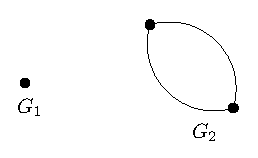
\includegraphics{bi-euler}
\caption{Los grafos más pequeños conexos y tal que sus vértices tienen grado par.}
\label{fig:bi-euler}
\end{figure}

  \HI Supongamos como hipótesis de inducción que cualquier grafo conexo cuyos vértices tienen grado par y que tiene menos de $n$ aristas tiene un ciclo Euleriano.
  
  \TI Sea $G$ un grafo conexo cuyos vértices tienen grado par y que tiene exactamente $n$ aristas. 
  Dado que ya mostramos en la BI los casos en que $G$ tiene sólo uno o dos vértices, podemos concentrarnos en los casos en que $G$ tiene al menos $3$ vértices distintos.
  Dado que $G$ es conexo y tiene al menos tres vértices, necesariamente debe existir un camino de largo 2 con aristas $e_1$ y $e_2$, que contiene tres vértices, digamos $v_1$, $v_2$ y $v_3$, un diagrama de esto se ve en la figura~\ref{fig:ti-euler1}.
  
  \begin{figure}[h!]
  \centering
  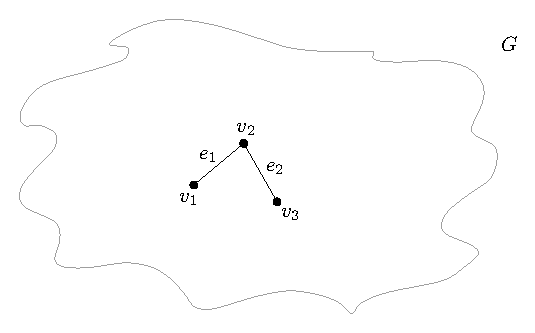
\includegraphics{ti-euler1}
  \caption{Camino de largo $2$ en un grafo con al menos $3$ vértices.}
  \label{fig:ti-euler1}
  \end{figure}
  
  Podemos crear un nuevo grafo $G'$ a partir de eliminar las aristas $e_1$ y $e_2$ de $G$, y agregar una nueva arista $e$ entre los vértices $v_1$ y $v_3$.
  Un diagrama de $G'$ se ve en la figura~\ref{fig:ti-euler2}.
  \begin{figure}[h!]
  \centering
  \includegraphics{ti-euler2}
  \caption{Creación de $G'$ a partir de la eliminación de $e_1$ y $e_2$ y la inserción de $e'$.}
  \label{fig:ti-euler2}
  \end{figure}
  La primera observación es que $G'$ tiene estrictamente menos aristas que $G$.
  Otra cosa que se puede observar es que los únicos vértices que pudieron haber visto afectados sus grado en $G$ son $v_1$, $v_2$ y $v_3$.
  Tanto para $v_1$ y $v_3$ su grado en $G'$ es el mismo que en $G$, para $v_2$ el grado se ha disminuido en $2$, por lo que, dado que en $G$ los tres vértices tenían grado par, en $G'$ también ocurrirá que tienen grado par y por lo tanto $G'$ tiene todos sus vértices de grado par.
  En este punto ``casi'' podemos aplicar la hipótesis de inducción a $G'$, dado que no tenemos seguridad que después del cambio, $G'$ sea un grafo conexo. 
  Nos pondremos entonces en ambos casos, cuando $G'$ resulta ser conexo y cuando no.
  Si $G'$ es conexo entonces cumple con la HI y por lo tanto tiene un ciclo Euleriano digamos $C'$ que contiene a todas las aristas de $G'$ y por lo tanto contiene a $e$, o sea $C'$ es un ciclo Euleriano en $G'$ que contiene la subsecuencia $(v_1,e,v_3)$.
  A partir de $C'$ podemos generar un ciclo para $G$ eliminando la arista $e$ y añadiendo las aristas $e_1$ y $e_2$, o sea cambiando la secuencia $(v_1,e_,v_3)$ de $C'$ por la secuencia $(v_1,e_1,v_2,e_2,v_3)$ este nuevo ciclo es claramente un ciclo que contiene todas las aristas de $G$, por lo tanto $G$ tiene un cilco Euleriano.
  Un diagrama de esta construcción se ve en la figura~\ref{fig:ti-euler3}.
  \begin{figure}[h!]
  \centering
  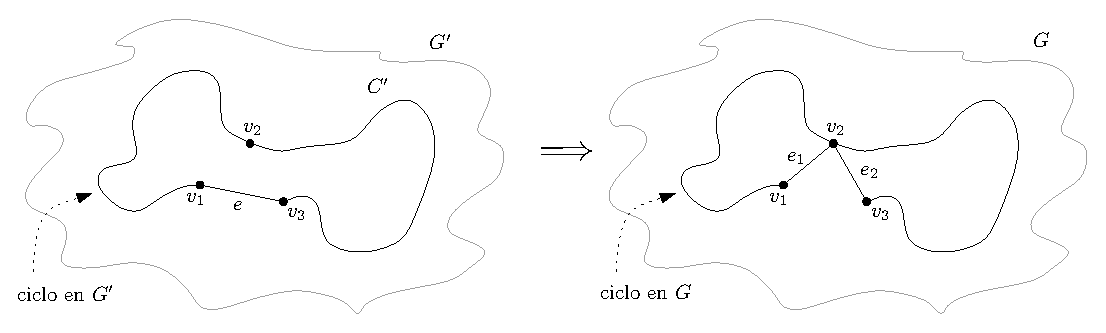
\includegraphics[width=\textwidth]{ti-euler3}
  \caption{Construcción de un ciclo Euleriano para $G$ a partir de uno para $G'$}
  \label{fig:ti-euler3}
  \end{figure}
  
  Si por otra parte $G'$ no es conexo, dado que $G$ es conexo, $G'$ tendrá dos componentes conexas, una que contendrá a $v_2$, y otra que contendrá a $v_1$ y $v_3$.
  Cada una de estas componentes tendrá sólo vértices de grado par y estrictamente menos aristas que $G$, por lo tanto a cada componente se le aplica la HI.
  Por HI entonces existe un ciclo, digamos $C'$ que podemos suponer que comienza y termina en $v_2$ y contiene a todas las aristas de una de las componentes de $G'$, o sea $C''$ es una secuencia de la forma $(v_2,\ldots,v_2)$.
  Por HI también existe otro ciclo $C''$ que pasa por todas las aristas de la otra componente de $G'$ y que por lo tanto contiene a $e$, o sea $C''$ contiene la subsecuencia $(v_1,e,v,3)$.
  Podría entonces crearse un ciclo para $G$ ``insertando'' $C'$ en $C''$ entre $v_1$ y $v_3$ añadiendo las aristas $e_1$ y $e_2$.
  Un diagrama de esta construcción se ve en la figura~\ref{fig:ti-euler4}.
  
  \begin{figure}[h!]
  \centering
  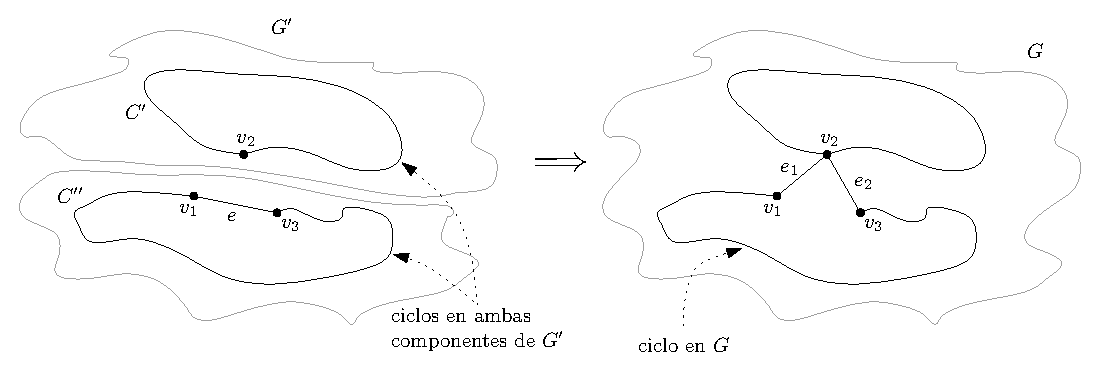
\includegraphics[width=\textwidth]{ti-euler4}
  \caption{Construcción de un ciclo Euleriano para $G$ a partir de los ciclos en las dos componentes de $G'$}
  \label{fig:ti-euler4}
  \end{figure}
  
  Por inducción se sigue entonces que cualquier grafo conexo cuyos vértices tiene todos grado par es Euleriano, o sea, contiene un ciclo Euleriano.
\end{inducciondemo}
\end{demostracion}
\end{teorema}

El alumno debiera notar que la demostración además nos entrega un algoritmo para encontrar un ciclo Euleriano en un grafo.
El algoritmo inicialmente realizaría el paso de cambiar un par de aristas por una sola como en la figura~\ref{fig:ti-euler2} y recursivamente debiera encontrar los ciclos del grafo resultante para luego construir un ciclo para el grafo inicial.
Los casos base serían un grafo con un único vértice a con grafo con dos vértices y dos aristas.

\begin{ejemplo}
Supongamos que se tiene un tablero de ajedrez de $n\times n$
>Existe algún valor de $n$ para el cuál el caballo pueda moverse desde un casillero, hacer todas las movidas que son posibles para él en el tablero una vez cada una y volver al casillero inicial?
La respuesta es no, el problema puede modelarse como un grafo, cada casillero representa un vértice y cada movida posible del caballo una arista.
Lo que se quiere entonces es encontrar un ciclo Euleriano.
No es difícil notar que para ningún $n$ (excepto claro $n=1$ existirá un ciclo Euleriano.
Los casos $n=2$ y $n=3$ resultan en grafos no conexos y para $n\leq 4$ el vértice correspondiente a la posición $(1,2)$ del tablero tiene grado $3$, luego existe un vértice de grado impar y por lo tanto no existirá un ciclo Euleriano.
\end{ejemplo}

La siguiente definición relaja un poco la noción de ciclo Euleriano.

\begin{definicion}
Un {\bf camino Euleriano} en un grafo $G$ es un camino no cerrado (el vértice inicial es distinto al final) que contiene a todos los vértices y a todas las aristas de $G$.
Recuerde que para ser un camino, no debe repetir aristas de $G$.
\end{definicion}

\begin{ejemplo}
El grafo de la figura~\ref{fig:graph23} no tiene un ciclo Euleriano ya que por ejemplo el vértice $v_3$ tiene grado 3, pero si tiene un camino Euleriano, de hecho el camino $(v_3,v_2,v_1,v_5,v_2,v_4,v_3,v_5,v_4)$ contiene a todos los vértices y a todas las aristas.
\begin{figure}[h!]
\centering
\includegraphics{graph23}
\caption{Un grafo que contiene un camino Euleriano.}
\label{fig:graph23}
\end{figure}
\end{ejemplo}

La noción de camino Euleriano captura mucho más nuestra intuición de ``poder dibujar una figura sin levantar el lápiz'', >existirá alguna caracterización para grafos que tengan caminos Eulerianos?
La respuesta es sí y la establecemos en el siguiente teorema.

\begin{teorema}
Un grafo $G$ tiene un camino Euleriano si y sólo si es conexo y contiene exactamente dos vértices de grado impar.

\begin{demostracion}
%Se dará la idea simplemente, los detalles de la demostración se dejan como ejercicio.
$(\Leftarrow)$ Supongamos que en un grafo conexo hay dos vértices de grado impar, digamos $u$ y $v$.
Si al grafo se le agrega una nueva arista para unir $u$ con $v$, el grafo resultante tiene todos sus vértices de grado par por lo que, por el teorema~\ref{teo:euler}, existirá un ciclo Euleriano en él.
Si a este ciclo se le ``borra'' la arista recién agregada resulta un camino que pasa por todos los vértices y aristas del grafo original, o sea un camino Euleriano.

$(\Rightarrow)$ 
Primero si en el grafo existe un camino Euleriano, entonces el grafo es necesariamente conexo (existe un camino entre cada par de vértices).
Supongamos ahora que el camino Euleriano parte en un vértice $v$ y termina en $u$, entonces al agregar una arista nueva $uv$ al camino, se forma un nuevo grafo que contiene un ciclo Euleriano (se cierra el camino).
Por el teorema~\ref{teo:euler} el nuevo grafo necesariamente tiene todos sus vértices de grado par, por lo que en el grafo inicial los únicos vértices de grado impar eran $u$ y $v$, por lo tanto el grafo tiene exactamente dos vértices de grado impar.
\end{demostracion}
\end{teorema}

\subsection{Ciclos Hamiltonianos}

Considere los grafos de la figura~\ref{fig:graph24}
>Es posible encontrar en alguno de ellos, un ciclo que contenga a todos los vértices una véz a cada uno (excepto por el inicial y final)?
Después de probar un poco nos damos cuenta de que en $G_1$ si existe tal ciclo, por ejemplo $(v_1,v_2,v_3,v_4,v_5,v_1)$, pero que en $G_2$ y en $G_3$ es imposible encontrar un ciclo de estas características.
\begin{figure}[h!]
\centering
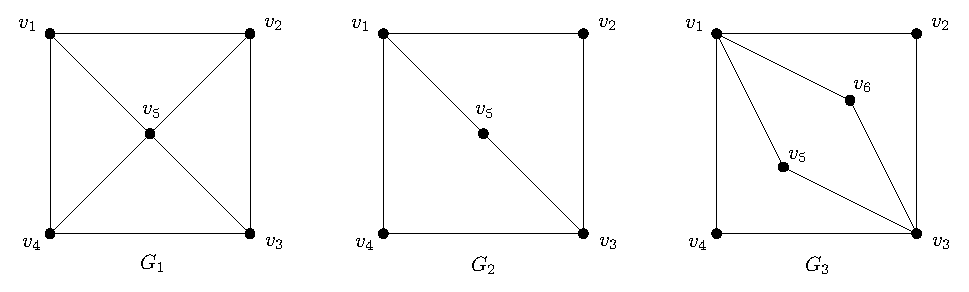
\includegraphics{graph24}
\caption{Solo $G_1$ tiene un ciclo Hamiltoniano.}
\label{fig:graph24}
\end{figure}

\begin{definicion}
Un ciclo en un grafo $G$ se dice {\bf ciclo Hamiltoniano} si contiene a todos los vértices de $G$ una única vez a cada uno (excepto por el vértice inicial y final).
A un grafo que contenga un ciclo Hamiltoniano lo llamaremos {\bf grafo Hamiltoniano}.
\end{definicion}

Con esta definición podemos decir que el grafo $G_1$ de la figura~\ref{fig:graph24} es Hamiltoniano, pero que los grafos $G_2$ y $G_3$ de la misma figura no lo son.
Una primera pregunta que podemos hacernos, dada la similitud del problema, es si existe alguna relación entre grafos Eulerianos y grafos Hamiltonianos.
Rápidamente podemos darnos cuenta que no hay una relación directa, por ejemplo, en la figura~\ref{fig:graph24} el grafo $G_1$ es Hamiltoniano pero no Euleriano, $G_2$ no es ni Hamiltoniano ni Euleriano, y $G_3$ es Euleriano pero no Hamiltoniano.

>Existirá alguna propiedad simple de chequear para determinar si un grafo es o no Hamiltoniano?
Hasta el día de hoy nadie ha sido capaz de encontrar una tal propiedad y es bastante poco probable que se encuentre.
Por otra parte nadie ha podido demostrar que no exista una propiedad simple de chequear.
Desde el punto de vista computacional lo anterior nos quiere decir que no existe un procedimiento rápido para determinar si un grafo cualquiera es o no Hamiltoniano, estamos condenados a tener que probar todas las posibilidades para poder responder SI o NO.
La verdad es que si la respuesta es SI, posiblemente no tengamos que probar todas las posibilidades basta con que encontremos un ciclo Hamiltoniano para que nuestra búsqueda acabe, el tema es que si la respuesta es NO, tendremos que asegurarnos de que ninguna posibilidad nos entrega un ciclo Hamiltoniano.
Este es un contraste radical con el de determinar si un grafo es Euleriano, para lo que sabemos que existe un algoritmo muy simple y rápido que responde SI o NO.
El problema de determinar si un grafo tiene o no un ciclo Hamiltoniano es un problema \emph{computacionalmente difícil} y se cree que no puede ser resuelto de manera \emph{eficiente} por un computador.
Más adelante en nuestro estudio nos enfocaremos con más detalle en este tipo de problemas y formalizaremos las nociones de \emph{eficiencia} y \emph{dificultad computacional}.

\begin{ejemplo}
Supongamos que se tiene un tablero de ajedrez de $n\times n$
>Para qué valores de $n$ puede un cabello moverse partiendo de un casillero cualquiera, pasando por todos los otros casilleros una única vez por cada uno y volviendo al casillero inicial?
Nuevamente el problema puede modelarse como un grafo, cada casillero representa un vértice y cada movida posible del caballo una arista. 
El problema se resume a determinar si el grafo resultante es o no Hamiltoniano.
Puede demostrarse que el grafo resultante es Hamiltoniano para todo $n$ par mayor o igual a $6$, sin embargo no hay una propiedad simple de chequear para asgurar esto (como en el caso de un ciclo Euleriano) y la demostración debe ser realizada por separado para cada caso.
\end{ejemplo}